\chapter{Introduction}
\label{cap1} \vspace{-1cm}

%
%\begin{flushright}
%\begin{minipage}{0.7\linewidth}
%\emph{``Em verdade, em verdade vos digo: quem ouve a minha palavra e
%cr� naquele que me enviou tem a vida eterna, n�o entra em ju�zo, mas
%passou da morte para a vida.''}
%\end{minipage}
%\end{flushright}
%
%\begin{flushright}
%{Jo 5:24}
%\end{flushright}

\section{Motivation}\label{motivation}

In nature it is possible to observe data fusion in a variety of phenomena. Animals combine signals from different senses, such as sight, hearing, smell, taste and touch, to recognize the surroundings. Plants have analogous mechanisms, which are used to modulate water consumption, to change the color of its leaves or to bend its structure towards the light, for instance. Throughout history, the sensory systems in living beings have evolved to assimilate multiple information coming from numerous sources in a highly complex and efficient way, in order to have a better perception of the environment. 

Nowadays information fusion is studied in many fields of science, as a way of exploiting data from multiple sources to achieve better outcomes in comparison to those obtained if any of the sources were used separately \citep{Dasarathy2001}. Other terms have been used to denote the synthesis of information in technical literature, for instance, data fusion, sensor fusion, multi-sensor fusion or multi-sensor integration. To avoid confusion, the terminology used by \citep{Elmenreich2002} will be adopted, whereby information fusion is understood as the overall term and sensor fusion is used in cases for which the sources of information are sensors. 

Some research fields have been increasingly exploiting the advantages of sensor fusion techniques, such as robotics, military, biometrics and image processing. The main benefits expected are related to accuracy, due to the use of redundant or complimentary data, to dimensionality, that is additional information being created by a group of data, and to robustness against failure and interference. Consequently much effort has been put into the development and investigation of data fusion techniques. The work of \citep{Khaleghi2013} presents an extensive review of different approaches available, categorizing them by the way sensor data uncertainty is represented, namely, probabilistic fusion, evidential belief reasoning, fuzzy reasoning, possibilistic fusion, rough set-based fusion and hybrid fusion. 
%\todo[caption={Resposta sobre coment�rio do Prof. Bruno}, inline]{COMENT�RIO: O que quer dizer com complimentary? RESPOSTA: Redundant e complementary data melhoram a acur�cia da informa��o de formas diferentes. Redundant seria quando um mesmo fen�meno fosse observado por v�rios sensores do mesmo tipo. Complementary � quando informa��es de tipo diferentes s�o usados}

Data fusion techniques based on probability theory are the earliest available and perhaps the most popular until now. They are concerned with estimating the probability distribution functions (PDF) of the system states by means of the Bayesian approach. If the system is linear and Gaussian, then the Kalman filter (KF) guarantees optimal estimation. For nonlinear processes, KF generalizations were proposed, such as the extended Kalman filter (EKF) or the unscented Kalman filter (UKF) \citep{Julier2004}. On the other hand, particle filters (PF) can be used to deal with both nonlinearities in the dynamics and non-Gaussian distributions \citep{Arulampalam2002}.

The most common class of systems studied in state estimation is the class of sampled-data systems, due to the wide use of digital devices. Although often described by continuous time differential equations, they can be modeled using discrete state equations, using approximation techniques \citep{Phillips1995}. Usually the sampling period of such systems are constant and known. In other words, the sensors are considered to transmit data at regular intervals. However, for many applications, such assumption is not valid. The use of several redundant sensors, for example, with different sampling rates or unsynchronized with one another, leads to data being received at irregular instants. Additionally, when data from multiple sensors are transmitted through several subsystems in a network, there might be loss of packets and delays \citep{Schenato2007} or even multiple information arriving simultaneously \citep{Moayedi2011}. In networked control systems, event-triggered sampling schemes have been proposed to optimize the access to communication channels \citep{Hu2017}, which will also generate time-varying sampling intervals. Nowadays, because of the ever-growing scientific advances, the technology of microprocessors, sensors and communication has become increasingly accessible, which continues to ensure that multiple sensor networks are more and more common.

Thus, despite improving accuracy and robustness of the estimation process, the fusion of data from multiple sensors might introduce challenges to the state estimation algorithms, due to sampling irregularities. Depending on how they take place, modifications to the KF and its generalizations can be carried out to tackle these abnormalities. In the work of \citep{Fatehi2017}, a fusion KF is proposed to estimate the states of a system with multi-rate measurements, whereby one of them is fast, regular and delay-free and the other is slow, irregular and randomly delayed. One application of such system is for industrial process control, where there is online instrumentation characterized by the former and data from laboratory analysis, which are much more accurate. For a more general case, when the random delays of are unknown, the work of  \citep{Gopalakrishnan2010} presents a critical analysis of the available methods for data fusion. They are separated into two categories: those that incorporate the delayed measurements upon arrival, and methods that rely in state augmentation, in order to assimilate the delayed information between estimation steps. 

In general the proposed methods and their performance will depend on particularities of the sampling irregularities and how they are modeled. Time delays can be multiple of a base sampling period, for instance. In those cases, the system can be described by a time-invariant discrete state equation, but with a particular representation of the measurement model. Delays can happen at single or multiple lags \citep{Penarrocha2012}, can lead to out-of-sequence measurements \citep{Anxi2005, Westenberger2013} or there can also be data dropout \citep{Zhu2013}. Nevertheless, the system can still be considered to be sampled at regular intervals. However, when the measurement instants take place after random time intervals, the discrete-state representation leads to a time-varying system, since the sampling period changes over time. Some researches treat the variable measurement instants as stochastic processes \citep{Micheli2002} or as a periodic sampling interval subject to noisy perturbations \citep{Shen2016}. Most of the time, the instant is considered to be known and the methods assimilate such information in the algorithm.

To the best of the author's knowledge, no method was proposed so far to take the irregularity into account and improve the estimation efficiency, for the cases in which the random time instant the signal was measured is not known or not reliable. If the sampling irregularity is caused due to the lack of sensor synchronization in the network, several algorithms can ensure a common timescale \citep{Sivrikaya2004}, at the expense of additional investments or energy use. Another approach, believed to be largely used on practice, is to disregard the irregularities, assimilating the measurements once they arrive, \emph{FALTA REFER�NCIA (dificuldade em encontrar)}. In this case, additional noises are tuned in the estimation process, but it might be irrelevant to the overall performance.

Knowing to what extent the estimation accuracy is deteriorated by ignoring the additional uncertainty caused by the sampling irregularity is important to decide whether or not to invest in synchronization. In addition, the investment in more sensors to the network in order to improve accuracy might not pay off, if it increases the occurrence of irregularities. Nevertheless there are no detailed studies on the behavior of the degradation in accuracy due to not addressing properly the irregularity in the sampling process. Therefore, this work assesses the differences in state estimation performance for systems with random sampling intervals with and without timestamp for different scenarios. The purpose is to shed some light on the trade-off for investments in sensor networks and synchronization.

\section{Problem Formulation}\label{problem-formulation} 

Consider the stochastic nonlinear sampled system
	
\begin{equation}\label{eq:processo}
\dot{x}(t)=f(x(t), u(t), w(t), t),
\end{equation}
\begin{equation}\label{eq:obs}
y(t_k)=g(x(t_k- \delta_{t_k}) ,v(t_k), t_k),
\end{equation}
\\
\noindent
where 	$f\!\!: \mathbb{R}^n \times \mathbb{R}^p \times \mathbb{R}^q \times \mathbb{R^+} \rightarrow \mathbb{R}^n $ and $g\!\!: \mathbb{R}^n \times \mathbb{R}^r \times \mathbb{R^+} \rightarrow \mathbb{R}^m $ are, respectively, the process and observation models, assumedly known. We assume that for all $k \geq 1$, the observations $y(t_k) \in \mathbb{R}^m$ and the first two moments of the random variables $x_0$ and $v(t_k)$ are known, where $x_0 \in \mathbb{R}^n$ is the initial state vector and $v(t_k) \in \mathbb{R}^r$ is the observation noise. Observations are taken at random time instants $t_k$ and are considered to be sorted ($t_{k+1}>t_k,\forall k \in \mathbb{N^+}$) and defined by the time intervals $h_0 \triangleq t_1$, $h_k \triangleq t_k-t_{k-1}, \ \forall k \geq 1$. In this work, we assume that the observation time instants $t_k$ are given by a Poisson random process. That is, the time intervals $h_k$ are independent and identically distributed exponential random variables with a known parameter $\lambda_{h_k}$, that is $h_k \sim \mathcal{E} (\lambda_{h_k})$,  where $\mathcal{E} (\lambda)$ defines an exponential PDF, with parameter $\lambda$, which is also its expected value. An example of time intervals produced by such a random process is illustrated in Figure \ref{fig:amost}.


\begin{figure}[h]
	\centering
	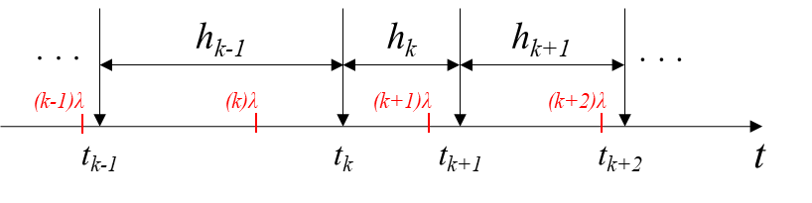
\includegraphics[scale=1]{Imagens/processo_amost}
	%\setlength{\belowcaptionskip}{-12pt}
	\caption[poisson]{Irregular sampling process modeled by a Poisson random process. Regularly spaced time intervals $\lambda$ are shown in red. An example of time instants $t_k$ realization is also shown, with the respective random time intervals $h_k$. The expected value of time interval is given by $E(h_k)=\lambda$.}
	\label{fig:amost}
\end{figure}

This sampling model characterizes a common application for an event-based sampling scheme or for a networked control system with unsynchronized sensors. \citep{Micheli2002}, for instance, considers a set of $N$ identical sensors measuring the state variables of a physical process every $L$ seconds. They prove that, if the sensors are independent and unsynchronized and $N$ is big enough, the waiting time between the realization of two consecutive measurements can be approximated by an exponential random variable $\mathcal{E} (\lambda)$, where the parameter is given by $\lambda = N/L$.

Arrival times to the estimator may be delayed during transmission by a random time amount $\delta_{t_k}$, also given by exponential random variables, with parameter $\lambda_{\delta_{t_k}}$, according to Figure~\ref{fig:delay}. Out-of-sequence measurements (OOSM) are not considered in this work. We assume that, in case a delayed measurement is to arrive later than future measurements, it gets lost in transmission.


\begin{figure}[h]
	\centering
	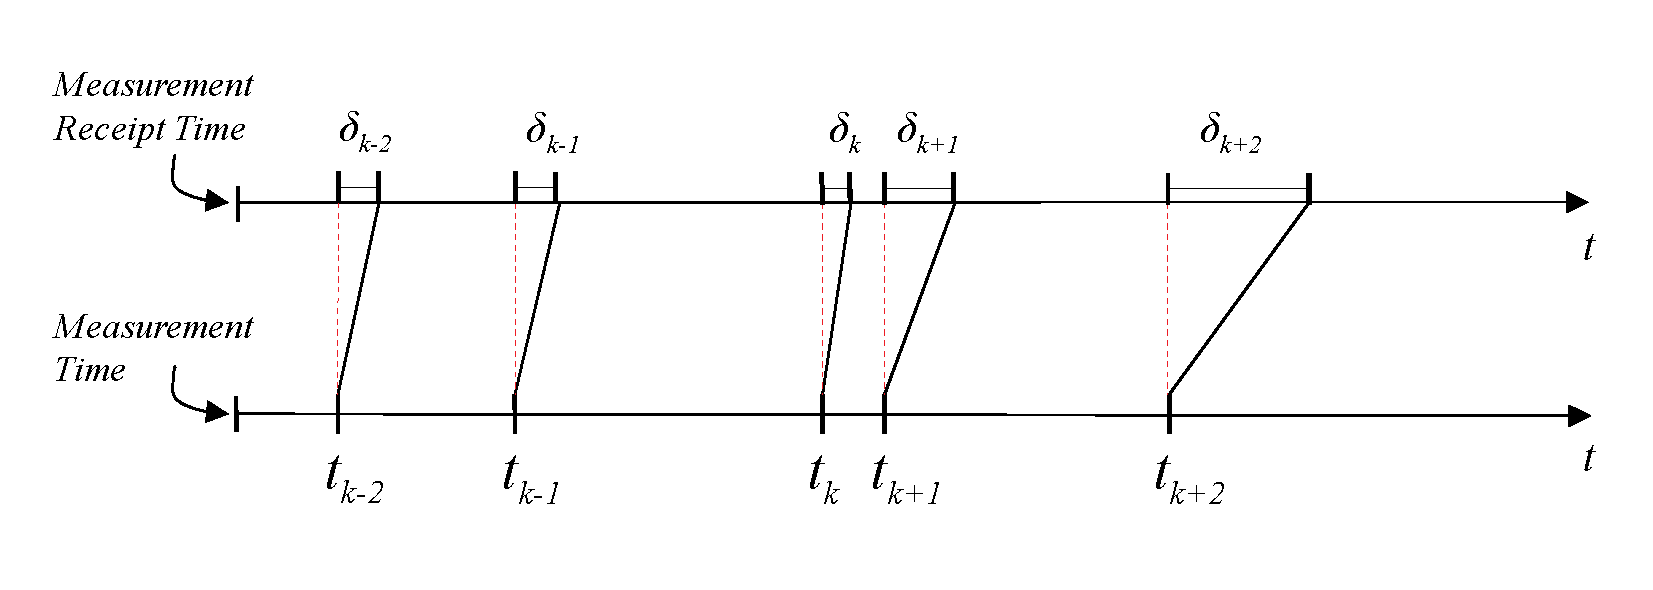
\includegraphics[width=1\textwidth]{Imagens/scheme-timedelay.pdf}
	%\setlength{\belowcaptionskip}{-12pt}
	\caption[poisson]{Randomly delayed measurements, modeled as exponential random variables. Random measurement times $t_k$ are received by the estimator after a random delay $\delta_{t_k}$}
	\label{fig:delay}
\end{figure}


Input data $u(t)$ are available at regularly spaced intervals $T$, that is $u(iT) \in \mathbb{R}^p$, $\forall i \geq 1$ are known.  $w(t) \in \mathbb{R}^q$ is process noise.

\duvida{Como tratar a quest�o do filtro cont�nuo para as entradas u(t)}

When time-stamp information is available, data assimilation can be performed at the correct measurement instants $t_k$. When they are not, the assimilation moment is considered to be the random receipt time instant or the next estimation moment, when there are no transmission time delays. 

We wish to estimate the state vector $x(t)$ and its covariance recursively, at regularly spaced time intervals $T$, given their initial values ($x_0$, $P_0$), the process model (\ref{eq:processo}), the input or control signals ($u(t): t \leq kT$) and the set of past observations $y(t_k): t_k - \delta_{t_k} \leq kT$. The knowledge of the time intervals $h_{k-1}: t_k - \delta_{t_k} \leq t$ is also taken into consideration when time-stamp information is available. We assume that the average time instant of observations $\lambda_{h_k}$ is greater than $T$ by a factor $\alpha>1$, i.e. $\lambda_{h_k}=\alpha T$. \duvida{A formula��o est� completa e matematicamente correta?}






\section{Objectives}\label{objectives}

1 frase para o objetivo geral
Objetivos espec�ficos

\section{Text Outline}\label{text-outline}



\clearpage

%
%\subsubsection{Problema 1: In}\label{sec:entrada_regular}
%
%\textit{As entradas $u(t)$ s�o medidas em intervalos regularmente espa�ados $T$, i.e. $u(iT) \in \mathbb{R}^p$, $\forall i \geq 1$ s�o conhecidas. $w(t) \in \mathbb{R}^q$ � o ru�do de processo. 
%}
%
%\subsubsection{Problema 2: Irregular input sampling}\label{sec:entrada_irregular}
%
%\textit{Medi��es feitas em instantes de tempo aleat�rios $t_{\textrm{u},i}$, $\forall i \in \mathbb{N^+}$, ordenados ($t_{\textrm{u},i+1}>t_{\textrm{u},i}$, $\forall i \in \mathbb{N^+}$) e definidos pelos intervalos de tempo $h_{\textrm{u},0} \triangleq t_{\textrm{u},1}$ e $h_{\textrm{u},i} \triangleq t_{\textrm{u},i}-t_{\textrm{u},i}, \ \forall i \geq 1$. $u(t_{\textrm{u},i}) \in \mathbb{R}^p$, $\forall i \geq 1$ s�o conhecidas. $w(t_{\textrm{u},i}) \in \mathbb{R}^q$ � o ru�do de processo. Assim como para a medi��o irregular da sa�da, os instantes de tempo $t_{\textrm{u},i}$ s�o dados por um processo aleat�rio de Poisson com par�metro $\lambda_u=T$, sendo $T$ o valor esperado do intervalo de tempo $h_{\textrm{u},i}$.
%}
%
%\subsubsection{Problema 2: Irregular sampling with time delay}\label{sec:entrada_irregular}
%\hfill 
%

